% Created 2015-02-04 Wed 13:50
\documentclass[presentation]{beamer}
\usepackage[utf8]{inputenc}
\usepackage[T1]{fontenc}
\usepackage{fixltx2e}
\usepackage{graphicx}
\usepackage{longtable}
\usepackage{float}
\usepackage{wrapfig}
\usepackage{rotating}
\usepackage[normalem]{ulem}
\usepackage{amsmath}
\usepackage{textcomp}
\usepackage{marvosym}
\usepackage{wasysym}
\usepackage{amssymb}
\usepackage{hyperref}
\tolerance=1000
\usetheme{default}
\author{Michael Clear}
\date{4 Feb 2015}
\title{Introduction to Cryptography}
\hypersetup{
  pdfkeywords={},
  pdfsubject={},
  pdfcreator={Emacs 24.4.1 (Org mode 8.2.10)}}
\begin{document}

\maketitle
\newcommand{\fname}{\mathsf}
\begin{frame}[label=sec-1]{Cryptography}
\begin{itemize}
\item = "Secret writing" throughout most of its history.
\begin{itemize}
\item More precisely, "writing" with a hidden meaning - as opposed to steganography where the existence of the "writing" itself is hidden.
\end{itemize}
\item The idea is to make a message unintelligble except to the intended receiver.
\end{itemize}

\vspace{20pt}
\begin{itemize}
\item Up until the 1970's, the typical pattern was (\cite{cos433})
\begin{itemize}
\item Somebody creates a cipher.
\item They claim (or assume) the cipher is unbreakable.
\item Their enemy breaks the cipher using cryptanalysis.
\end{itemize}
\end{itemize}
\end{frame}
\begin{frame}[label=sec-2]{Two Periods: BDH and ADH}
\begin{itemize}
\item BDH - Before Diffie-Hellman < 1976
\item ADH - After Diffie-Hellman > 1976
\end{itemize}

\vspace{20pt}
\textbf{Two big changes in 1976}
\begin{itemize}
\item Selection of Data Encryption Standard (DES) block cipher.
\item Public-key cryptography - Diffie-Hellman.
\end{itemize}
\end{frame}

\begin{frame}[label=sec-3]{BDH: Symmetric Cryptography}
\begin{itemize}
\item A symmetric cipher uses the same key for encryption and decryption.
\item Two main types:
\begin{itemize}
\item Stream cipher.
\item Block cipher.
\end{itemize}
\item Prior to 1970's, most ciphers were stream ciphers.
\item A symmetric cipher consists of three algorithms - $G$, $E$ and $D$:
\begin{itemize}
\item $G$ generates a secret key $k$.
\item $E$ takes key $k$ and plaintext $m$ and ouputs a ciphertext $c$ i.e. $c = E(k, m)$.
\item $D$ takes a key $k$ and a ciphertext $c$ and ouputs a plaintext $m$ i.e. $m = D(k, c)$.
\end{itemize}
\end{itemize}
\end{frame}
\begin{frame}[label=sec-4]{Entropy}
\begin{itemize}[<+->]
\item Measure of uncertainty in a given source of information.
\item It measures the average amount of information contained in a given message, where a message is drawn from some distribution.
\item Shannon's definition of entropy $H$:
\begin{itemize}
\item Let $X$ be a discrete random variable.
\item Let $P(X)$ denote the probability mass function of $X$.
\item Define $H$ as $H(X) = -\sum_{i} P(x_i) \log_2{P(x_i)}$.
\end{itemize}
\item $H$ gives the average number of bits of information contained in some message, which we call the amount of \emph{entropy}.
\end{itemize}
\end{frame}
\begin{frame}[label=sec-5]{Unicity Distance}
\begin{itemize}[<+->]
\item Minimum length of ciphertext needed for a computationally unbounded adversary to recover the (unique) encryption key.
\item In a brute force attack where every key is tried, there should be just one key that decrypts to a sensible plaintext.
\item The keys other than the correct key that yield a sensible plaintext on decryption are called \emph{spurious keys}.
\item The unicity distance is the needed length of ciphertext for the number of spurious keys to be zero.
\item We calculate the unicity distance as:
\begin{itemize}
\item Let $k$ be the number of keys.
\item Let $s$ be the number of "sensible" (readable) plaintexts.
\item Let $p$ be the total number of possible plaintexts.
\item Then the unicity distance is the length of ciphertext $U$ such that $k \cdot \frac{s}{p} = 1$.
\end{itemize}
\end{itemize}
\end{frame}
\begin{frame}[label=sec-6]{Unicity Distance (Cont'd)}
\begin{itemize}[<+->]
\item We can alternatively define the unicity distance:
\begin{itemize}
\item Let $K$ be the key space. The entropy of $K$ is $H(K)$.
\item Let $H(M)$ be the entropy of a given "sensible" (e.g: English language) plaintext character.
\item Let $n$ be the number of bits per plaintext character.
\item Then we have $U = H(K) / (n - H(M))$.
\item The value $D = n - H(M)$ is the redundancy of the plaintext.
\end{itemize}
\end{itemize}
\end{frame}
\begin{frame}[label=sec-7]{Perfect Secrecy}
\begin{itemize}[<+->]
\item A cipher is perfectly secure if the entropy of the plaintext \emph{given} the ciphertext is equivalent to the entropy of the plaintext.
\begin{itemize}
\item Let $H(M)$ be the entropy of the plaintext.
\item Let $C$ be the probability distribution of the ciphertext.
\item Then 
\begin{equation*}
H(M) = H(M \mid C)
\end{equation*} where $H(M | C)$ is the \emph{conditional entropy} of $M$ given a ciphertext from $C$.
\item Put another way, for all plaintexts $m \in M$ and all ciphertexts $c \in C$, we have
\begin{equation*}
 \fname{Pr}(m) = \fname{Pr}(m \mid c)
\end{equation*}
\end{itemize}
\end{itemize}
\end{frame}
\begin{frame}[label=sec-8]{One-time Pad}
\begin{itemize}[<+->]
\item Described by Gilbert Vernam in 1917. Known as the Vernam Cipher.
\item A stream cipher in which the key is the same length as the plaintext, and is chosen to be truly random.
\item The random key is called a pad.
\item The cipher is unbreakable as long as the key is
\begin{itemize}
\item truly random
\item kept secret
\item used only once
\item the same length as the plaintext.
\end{itemize}
\item The one-time pad has perfect secrecy.
\item The $n$-th character is enciphered by "adding" the $n$-the character of the key to the $n$-th character of the plaintext.
\item Example: using addition modulo $2$ (XOR) when encrypting a binary message.
\end{itemize}
\end{frame}
\begin{frame}[label=sec-9]{Confusion and Diffusion}
\begin{itemize}[<+->]
\item Encryption is based on the principles of confusion and diffusion.
\item \textbf{Confusion: } Making the relationship between the ciphertext and the key complex. Each ciphertext character should depend on several different parts of the key.
\begin{itemize}
\item Means that drastic changes are made from the input to the output.
\item Can be achieved via the technique of substitution.
\end{itemize}
\item \textbf{Diffusion: } Changing a single character of the plaintext changes many characters of the ciphertext.
\begin{itemize}
\item Distributing the statistical structure of the plaintext across much larger structures in the ciphertext.
\item Can be achieved via the technique of permutation (aka transposition).
\end{itemize}
\end{itemize}
\end{frame}
\begin{frame}[label=sec-10]{Substitution}
\begin{itemize}[<+->]
\item Replace each character of the plaintext with a potentially different character determined by the key.
\item In a \emph{monoalphabetic} substitution cipher, the key decides the particular susbtitution table that is used.
\item Example - Caesar Cipher: each character is shifted by $k$ places in the alphabet where $k$ is the key.
\begin{itemize}
\item For $k$ = 3, the string "HELLO" is encrypted as "KHOOR".
\item Encryption of $m$ is $c = m + k \mod{26}$.
\end{itemize}
\item A monoalphabetic substitution cipher can have $P!$ different keys where $P$ is the number of plaintext characters.
\begin{itemize}
\item So English language text with 26 characters results in $26! = 403291461126605635584000000$ possible keys.
\item The entropy per character of English is $H(M) \approx 1.5$.
\item The unicity distance is $U = H(K) / (n - H(M)) = \log_2{26!} / (\log_2{26} - 1.5) \approx 28$.
\end{itemize}
\end{itemize}
\end{frame}
\begin{frame}[label=sec-11]{Frequency Analysis}
\begin{itemize}[<+->]
\item A monoalphabetic substitution cipher can be defeated with frequency analysis.
\item Invented by Al-Kindi in the 9th century.
\item Involves counting the number of occurences of each ciphertext character and matching against the frequency distribution of plaintext characters.
\item In English, the most frequently occuring letters are (in order) E, T, A, O, I, N, S, H, R, D, L, U\ldots{}
\item So given a ciphertext generated from an English plaintext, the most frequently occuring character likely corresponds to E etc.
\end{itemize}
\end{frame}

\begin{frame}[label=sec-12]{Polyalphabetic Substitution Cipher}
\begin{itemize}[<+->]
\item Uses multiple substitution alphabets.
\item The main idea is to change the substitution alphabet with each plaintext character, so the first letter is encrypted according to one alphabet, the second according to a different alphabet and so on (note the alphabets may repeat after a certain period).
\end{itemize}
\end{frame}
\begin{frame}[label=sec-13]{Vigenère Cipher}
\begin{itemize}[<+->]
\item Example of a polyalphabetic substitution cipher.
\item Works as follows:
\begin{itemize}
\item Let $k$ be a keyword such as "BLAZE", with $n = 5$ letters.
\item Let $k_i$ denote the numeric value (modulo 26) of the $i$-th letter of the keyword $k$.
\item The $i$-th letter of plaintext $m_i$ is encrypted as $c_i = m_i + k_{i \pmod{n}} \pmod{26}$ (when represented modulo $26$)
\end{itemize}
\item Encrypting the text "HELLO" with keyword "BLAZE" yields the ciphertext "IPLKS".
\end{itemize}
\end{frame}
\begin{frame}[label=sec-14]{Viginère Cipher - Tabula Recta}
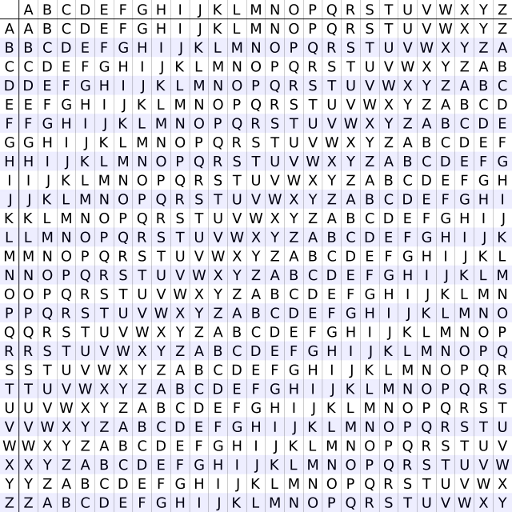
\includegraphics[scale=0.45]{tabula_recta.png}


Source: Wikipedia
\end{frame}
\begin{frame}[label=sec-15]{Transposition}
\begin{itemize}
\item Idea: rearrange the plaintext (change the order) to produce the ciphertext.
\item The positions of the plaintext characters are shifted.
\item Also known as \emph{permutation}.
\item Examples:
\begin{itemize}
\item Rail Fence
\item Route Cipher
\item Columnar Transposition
\end{itemize}
\end{itemize}
\end{frame}

\begin{frame}[label=sec-16]{Example: Columnar Transposition}
\begin{itemize}
\item Write plaintext along rows whose length is determined by the key
\item Example (here X denotes a null character):
\end{itemize}
\begin{center}
\begin{tabular}{lllll}
T & H & E & R & E\\
M & U & S & T & B\\
E & S & O & M & E\\
K & I & N & D & O\\
F & W & A & Y & O\\
U & T & O & F & H\\
E & R & E & X & X\\
\end{tabular}
\end{center}
\begin{itemize}
\item Suppose the key specifies the row length as 5 and the order of columns to write out as 4, 2, 5, 1, 3.
\item Then we get the ciphertext by writing out the columns in the specified order:
\begin{itemize}
\item we obtain: RTMDYFXHUSTWTREBEOOHXTMEKFUEESONAOE
\end{itemize}
\end{itemize}
\end{frame}
\begin{frame}[label=sec-17]{Example: Columnar Transposition (Cont'd)}
\begin{itemize}
\item The key could be alternatively given as a keyword such as TOWER
\begin{itemize}
\item the length of the keyword represents the row length.
\item the alphabetical order of the letters in the keyword gives the order of the columns to be written out.
\end{itemize}
\end{itemize}
\end{frame}
\begin{frame}[label=sec-18]{References}
\bibliography{crypto_intro}
\end{frame}
% Emacs 24.4.1 (Org mode 8.2.10)
\end{document}
